\documentclass[IN,11pt,openright,bachelor,english]{tumthesis}

% Include common packages
\usepackage{packages}

% IEEE tools for tweaking bib style
\usepackage{IEEEtrantools}

\newcommand\toc{\relax}

\usepackage[backend=bibtex]{biblatex}
\usepackage{booktabs}
\usepackage{tabularx}
\usepackage{longtable}
\usepackage{tabu}
\usepackage{ltxtable}
\usepackage{url}
\usepackage[style=base]{caption}
\captionsetup{%
	font={rm,footnotesize},
	labelfont={sc},
}
\captionsetup[subfloat]{%
	font={rm,footnotesize},
	labelfont={rm},
}
\usepackage{subfig}
\usepackage{nicefrac}
\usepackage{longtable}
\usepackage[hang]{footmisc}
\usepackage{acro}
\usepackage{blindtext}

\usepackage{graphicx}

\setlength\footnotemargin{5pt}

% Theorem environments
\newtheorem{definition}{Definition}
\newtheorem{theorem}{Theorem}
\newtheorem{example}{Example}
\newtheorem{lemma}{Lemma}


% hyphenation
\hyphenation{op-ti-cal net-work net-works semi-con-duc-tor tech-nique tech-niques}


\usepackage{mdframed}
\newlength{\charwidth}
\setlength{\charwidth}{\widthof{\scriptsize\texttt{x}}}

\makeatletter
\newenvironment{moeplstborder}[2][]{%
\ifx#1\@empty\@empty%
	\edef\@margin{-1.5\baselineskip}%
\else%
	\edef\@margin{#1}%
\fi%
\vspace{-\baselineskip}
\begin{center}
\begin{minipage}{#2}
\begin{mdframed}[%
	topline=false,leftline=false,bottomline=false,rightline=true,
	linecolor=TUMRed!20,linewidth=\charwidth,
	innertopmargin=\@margin,innerbottommargin=-0.5\baselineskip,
	innerleftmargin=0pt,innerrightmargin=-\charwidth,
	userdefinedwidth=#2,
]%
}%
{%
\end{mdframed}%
\end{minipage}
\end{center}
}%
\makeatother

% Needed for Bachelor's theses, Master's theses and IDP
\titleenglish{Performance Analysis of VPP}
\titlegerman{Performance-Analyse von VPP}
\author{Peter Okelmann}
\supervisor{\NEThead}
\advisor{}
\assistants{Paul Emmerich, Dominik Scholz}
\courseofstudy{Informatics}
\date{April 15, 2019}
\location{Garching}

\setcounter{tocdepth}{2}

\DeclareAcroListStyle{longtabu}{table}{%
	table = longtabu,
	table-spec = @{}>{}lX@{}
}{%

\acsetup{%
	list-style=longtabu,
	extra-style=plain,	% remove dot after long in list
	only-used=false,
}

\tabulinesep=1ex

\DeclareAcronym{iso}{
	short				= {\sc{ISO}},
	long				= {International Organization for Standardization},
	list				= {\acl{iso}.},
}
\DeclareAcronym{osi}{
	short				= {\sc{OSI}},
	long				= {Open Systems Interconnection},
	list				= {\acl{osi}.},
	extra				= {%
		Reference model for layered network architectures by the \ac{osi}.
	},
}
\DeclareAcronym{pdu}{
	short				= {\sc{PDU}},
	short-plural-form	= {\sc*{PDU}s},
	long				= {protocol data unit},
	long-plural-form	= {protocol data units},
	list				= {\Acl{pdu}.},
	extra				= {%
	Refers to a message at a specific layer of the \acs{osi} model including
	all headers and trailers of the respective layer and all layers above.
	},
}
\DeclareAcronym{sdu}{
	short				= {\sc{SDU}},
	short-plural-form	= {\sc*{SDU}s},
	long				= {service data unit},
	long-plural-form	= {service data units},
	list				= {\Acl{sdu}.},
	extra				= {%
		Refers to the payload of a message at a specific layer of the \acs{osi}
		model excluding all headers and trailers of the respective layer.
	},
}
\DeclareAcronym{mac}{
	short				= {\sc{MAC}},
	long				= {medium access control},
	list				= {\Acl{mac}.},
}
\DeclareAcronym{tcp}{
	short				= {\sc{TCP}},
	long				= {transmission control protocol},
	list				= {\Acl{tcp}.},
	extra				= {%
		Stream-oriented, reliable, transport layer protocol.
	}
}
\DeclareAcronym{udp}{
	short				= {\sc{UDP}},
	long				= {user datagram protocol},
	list				= {\Acl{udp}.},
	extra				= {%
		Datagram-oriented, unreliable transport layer protocol.
	}
}
\DeclareAcronym{sctp}{
	short				= {\sc{SCTP}},
	long				= {Stream Control Transmission Protocol},
	list				= {\acs{sctp}.},
	extra				= {%
		Datagram-oriented, semi-reliable transport layer protocol.
	}
}
\DeclareAcronym{vpp}{
	short				= {\sc{VPP}},
	long				= {Vector Packet Processing},
	list				= {\Acl{vpp}.},
	extra				= {%
		A fast software router.
	}
}
\DeclareAcronym{fdio}{
	short				= {\sc{FD.io}},
	long				= {the Fast Data Project},
	list				= {\Acl{fdio}.}
}
\DeclareAcronym{dpdk}{
	short				= {\sc{DPDK}},
	long				= {the Data Plane Development Kit},
	list				= {\Acl{dpdk}.},
	extra				= {%
		\url{https://www.dpdk.org/}
	}
}
\DeclareAcronym{dut}{
	short				= {\sc{DUT}},
	long				= {Device under Test},
	list				= {\Acl{dut}.}
}
\DeclareAcronym{fib}{
	short				= {\sc{fib}},
	long				= {Forwarding Information Base},
	list				= {\Acl{fib}.}
}
\DeclareAcronym{cli}{
	short				= {\sc{CLI}},
	long				= {Command Line Interface},
	list				= {\Acl{cli}.}
}
\DeclareAcronym{sdn}{
	short				= {\sc{SDN}},
	long				= {Software Defined Network},
	list				= {\Acl{sdn}.}
}

\addbibresource{bib/IEEEfull.bib}
\addbibresource{bib/litnew.bib}


%\renewcommand{\andothersdelim}{}
%bib.sty does not work older bibtex versions (works on TexLive 2016 or newer)
%\usepackage{bib}

% Load late to avoid same identifier warning
\usepackage[colorlinks=false,pdfborder={0 0 0}]{hyperref}


\begin{document}%

% Makes sure that same author names are not replaced by dahes
\bstctlcite{IEEEexample:BSTcontrol}

\pagenumbering{gobble}
\maketitle%
\cleardoublepage


\begin{abstract}
	\small

\blindtext

\blindtext

\end{abstract}

%\begin{thanks}
%%\input{/home/moepi/.thanks}
%\end{thanks}

%\begin{preface}
%foo bar
%\end{preface}

\tableofcontents
\listoffigures
\listoftables

\startcontent



\chapter{Introduction}

% microservices -> virtualization -> software routing
% problem: software router slower than specialized hardware

A world of microservices counting on virtualization is more and
more interested in being able to move dedicated hardware into
virtualized spaces. But especially high speed networking is
traditionally bound to specialized hardware, because many software
routers can't keep up performance-wise.

% solution: faster software routers like VPP
% vpp: cisco

There are software routers though which focus on performance and are
improved in many aspects. Especially frameworks like DPDK
\cite{inteldpdk} help in the making of fast software routers which can
run on affordable commodity hardware. One of the routers built on that
framework is \Ac{vpp} which was developed by Cisco and is now open
source and maintained by \Ac{fdio}. \Ac{vpp} can be virtualized and
has packet input nodes for NIC's handled by \Ac{dpdk} (dpdk-input),
but can also use virtual links like virtual Linux interfaces (tuntap,
af-packet-input, tapcli) or memory map based interfaces (memif,
netmap, vhost-user) which allow for good interoperability with local
virtualized systems. Therefore it is promising for highly virtualized
environments.

% little indepencent and comparable benchmarks of vpp and others

% therefore this work: well documented for comparison, automated for reproducability 

% tests shall 
% - find numerical answers to the performance question
% - make vpp comparable to other software routers
% - model to describe performance behaviour
% - indentify/quantify bottlenecks

There is little independent performance analysis of \Ac{vpp} though
and none that compares it to other software routers. Therefore this
work presents well documented \cite{my:repo} performance tests and
results of \Ac{vpp} in different scenarios to enable comparability to
other software routers. The tests procedures are as far as possible
automated, to be as reproducible as possible. The resulting data is
then analyzed to learn about the behavior of \Ac{vpp} and it's
performance bottlenecks.

% therefore the structure of this paper: 
% 1. previous performance analysis of routers in general and vpp in particular
% 2. analysis of performance critical aspects of software routing, benchmarking challenges and vpp
% 3. describe methodology and executed tests
% 4. evaluate results and create model

First, this paper will introduce related work about existing methods
for router performance analysis and about existing benchmarking
results for \Ac{vpp} in particular. Then challenges and performance
critical aspects of software routing and \Ac{vpp} are analyzed. In
section \ref{sec:methodology} the methodology and the executed tests
are described in detail. This paper presents measured performance for
scaling on multiple cores, impact of varying CPU clocks, IP version,
layer 2 \Ac{fib} and layer 3 \Ac{fib} sizes and tasks like \Ac{vxlan}
encapsulation. Finally the results are evaluated to create a model to
describe \Ac{vpp}'s performance behavior.



\section{Background}

\subsection{Core Features}

% features:
% - modularity, feature rich
% - vectorization
% - RSS
% - dpdk: fast userspace NIC drivers

Core features of \Ac{vpp} are... 

... it's vectorized processing of packets in badges as the name
indicates. This allows for better optimization.

... it's support for \Ac{dpdk} with it's fast user-space NIC drivers.

... it's modular packet processing graph. Specific features are
implemented in nodes for example like ip4-lookup, ip6-lookup or
vxlan4-encap and vxlan6-encap. Not only has it packet input nodes for
NIC's handled by \Ac{dpdk} (dpdk-input), but also drivers to virtual
links like virtual linux interfaces (tuntap, af-packet-input, tapcli)
or memory map based interfaces (memif, netmap, vhost-user). New
features can be added with plugins extending the packet processing
graph by new nodes, adding new processing paths and adding new CLI
commands. \cite{linguaglossa2017high}


\subsection{Releases}

% releases:

Each release (such as v18.10) contains the following pre-release
milestones:  With the first label "F0" the API is frozen and
development shall aim for stability. For the second label "RC1" only
bug fix changes are accepted and a first artifact is released. Then
the iteration repeats and a second "RC2" version is released. Those
pre- releases are marked with a tag containing the version number and
the iteration appendix (v18.10-rc1). The final release will have no
extra tags in their name. The git tag marks the official release, but
the version-specific branch can still receive occasional updates.
\cite{vppwiki:releases}

The oldest version of VPP available in the github repository is from
2016. Unless otherwise specified this performance analysis used the
v18.10 branch from 14th of december 2018\footnote{commit
a8e3001e68d8f5ea6cf526b131c92f5993597f81}.


\subsection{Use Cases}

% interesting scenarios / use cases: 

A developer once formulated the design goal of \Ac{vpp}: It shall seemlessly integrate into the existing \Ac{sdn} stacks and it shall "become the foundation of the future cloud native services" \cite{florincoras}. That is, because \Ac{vpp} can serve in quite some different scenarios and can connect to different control plane tooling. 

\paragraph{Data Plane}

% - routing the internet: >500.000 routes
% - scale to multiple cpu's
% - latency behaviour
% - more complex tasks like vxlan encapsulation

The internet the BGP table size grew to 512,000 prefixes in 2014 and
it continues growing. As \Ac{vpp} aims to be used for routing tasks,
it has to perform well with big routing tables.

For handling high loads \Ac{vpp} helps spreading the computation
intensive frame processing tasks to multiple cpu cores. Qosmos for
example uses \Ac{vpp} to implement deep packet inspection
\cite{qosmos}.

Viosoft on the other hand uses \Ac{vpp} in the context of embedded
systems which might require stable or short latencies \cite{viosoft}.
Therefore latency behaviour represents an important aspect of
performance analysis, too.

\paragraph{Control Plane}

OpenDaylight software can do some VPP management using an OpenFlow interface via LISP flow mapping (Locator ID Separation Protocol) \cite{opendaylight:lisp}. 

VPP also integrates into OpenStack Neutron, a networking management software for the OpenStack cloud computing platform.


vPE: 39 times in source code, 
- Cisco Virtual Multiservice Data Center (VMDC)
- vPE (Virtual Provider Edge) provides VMDC 1-4.x

vPE is used by 
Cisco VSG (Virtual Security Gateway)
Cisco ASA 1000v, a Cloud Firewall
Cisco vWAAS (Virtual Wide Area Applications Services)
Citrix ADC VPX, a SDN suite





\section{Related Work}

There has been a previous work analyzing and describing the design,
architechture and performance of \Ac{vpp} \cite{linguaglossa2017high}.
It presents measurement results mainly regarding very specific
properties like packet vector sizes but lacks results about the impact
of hash table sizes (l2fib, l3fib). This paper on the other hand ...

% TODO add differences. i haz:
% - l2fib, ip4/6 l3fib routing table entries
% - high core count cpu scaling
% - models describing performance behaviour
% - more in-depth latency description and model

There is also a repository \cite{github:vpp-bench} containing some
\Ac{vpp} startup and setup scripts used for
\cite{linguaglossa2017high}.

% moongen

Regarding benchmarking methodology, \cite{emmerich2015moongen}
discusses MoonGen, the load generator used in this paper.

% rfc2544 not usable

Unfortunately there is no fitting and established benchmarking
routine. Even though RFC2544 \cite{rfc2544} describes "Benchmarking
Methodology for Network Interconnect Devices", most of the suggestions
done in it, are not relevant or applicable to software routers like
\Ac{vpp}.

% frame sizes

For example it stresses procedures to test different ethernet frame
sizes. Frame size is no limiting factor inside the \Ac{dut} though (in
software routers with high packet rates) and is thus not necessary for
upper bound performance analysis. \cite{emmerich2015assessing}

% - "At the start of each trial a routing update
%    MUST be sent to the DUT." (long running, no good idea)

Furthermore the RFC states: "At the start of each trial a routing
update MUST be sent to the DUT" \cite{rfc2544}. Adding up to several
million routing entries using networking protocols before every test
run doesn't appear to be a feasable approach. Instead \Ac{vpp}'s CLI
is used to add all table entries using a single command.

% - each test-run SHOULD take over a minute. (no change after 20
%   seconds with turbo boost disabled) latency measurement one packet
% - per minute - to slow rate

Generally speaking, the RFC's requirements torwards the duration of
test runs exceeds what was done for this paper. According to the RFC a
test run should take longer than a minute - latency measurements shall
only measure timings of a single packet per minute. Providing a
constant level of CPU performance for example by disabling Intels
turbo-boost, \Ac{vpp} stabilizes after only 10 to 20 seconds of
receiving load which allows for way shorter test runs.

% this one uses definitions of rfc1242. 
% usable: throughput and latency

RFC 2544 uses some definitions from RFC1242 \cite{rfc1242} like
"Throughput": RFC 1242 defines throughput as the highest throughput
without any packet loss, which is not the same as the maximum
measurable throughput. This paper refferes to throughput as the
maximum measurable throughput if not specified otherwise.

% - latency measurement at the rfc1242 throughput rate -> doesnt work because of variance

% removed, because too complicated to be correct. 
% "moongen latency measurement is science stadtard" - paul
% RFC 1242's definition of latency conforms to the latency measured by
% MoonGen which was used for this paper. RFC 2544 on the other hand
% additionally requires to measure the latency at the throughput
% according to RFC 1242. As this paper will show, the latency at very
% high throughput rates without packet loss varies a lot. Instead in
% order to get comparable latency results, a lower packet rate has to be
% selected.

% TODO - special frames: broadcast, management, routing update
% mentioned in rfc, but not looked at in this paper



\section{Analysis}

% bring up features from #Background
% features:

\subsection{Experiment Setup}

Each device in the testbed has at least three active ethernet links:
One connecting it to a management server, and two connected to the
corresponding \Ac{dut} or loadgen (load generator). The management
server (kauas) uses pos tools to set boot images, boot, run setup and
testing scripts on the testbed devices and collect script output and
artifact files containing test results.

As figure \ref{setup} shows, each test contains two
devices. The \Ac{dut}, running \Ac{vpp}, and the loadgen, generating
packets and sending them to the \Ac{dut} to test \Ac{vpp}. \Ac{vpp}
then forwards the packets back to the loadgen which allows the loadgen
to create accurate throughput and latency measurments.

On the \Ac{dut} some debug information like error counts are beeing
gathered from the \Ac{vpp} CLI interface and Linux perf tools
\cite{perf} attach to the vpp process to collect time spent per symbol
and stats like cpu cycles or cache misses.

\begin{figure}[!ht]
\noindent\hspace{0.5mm}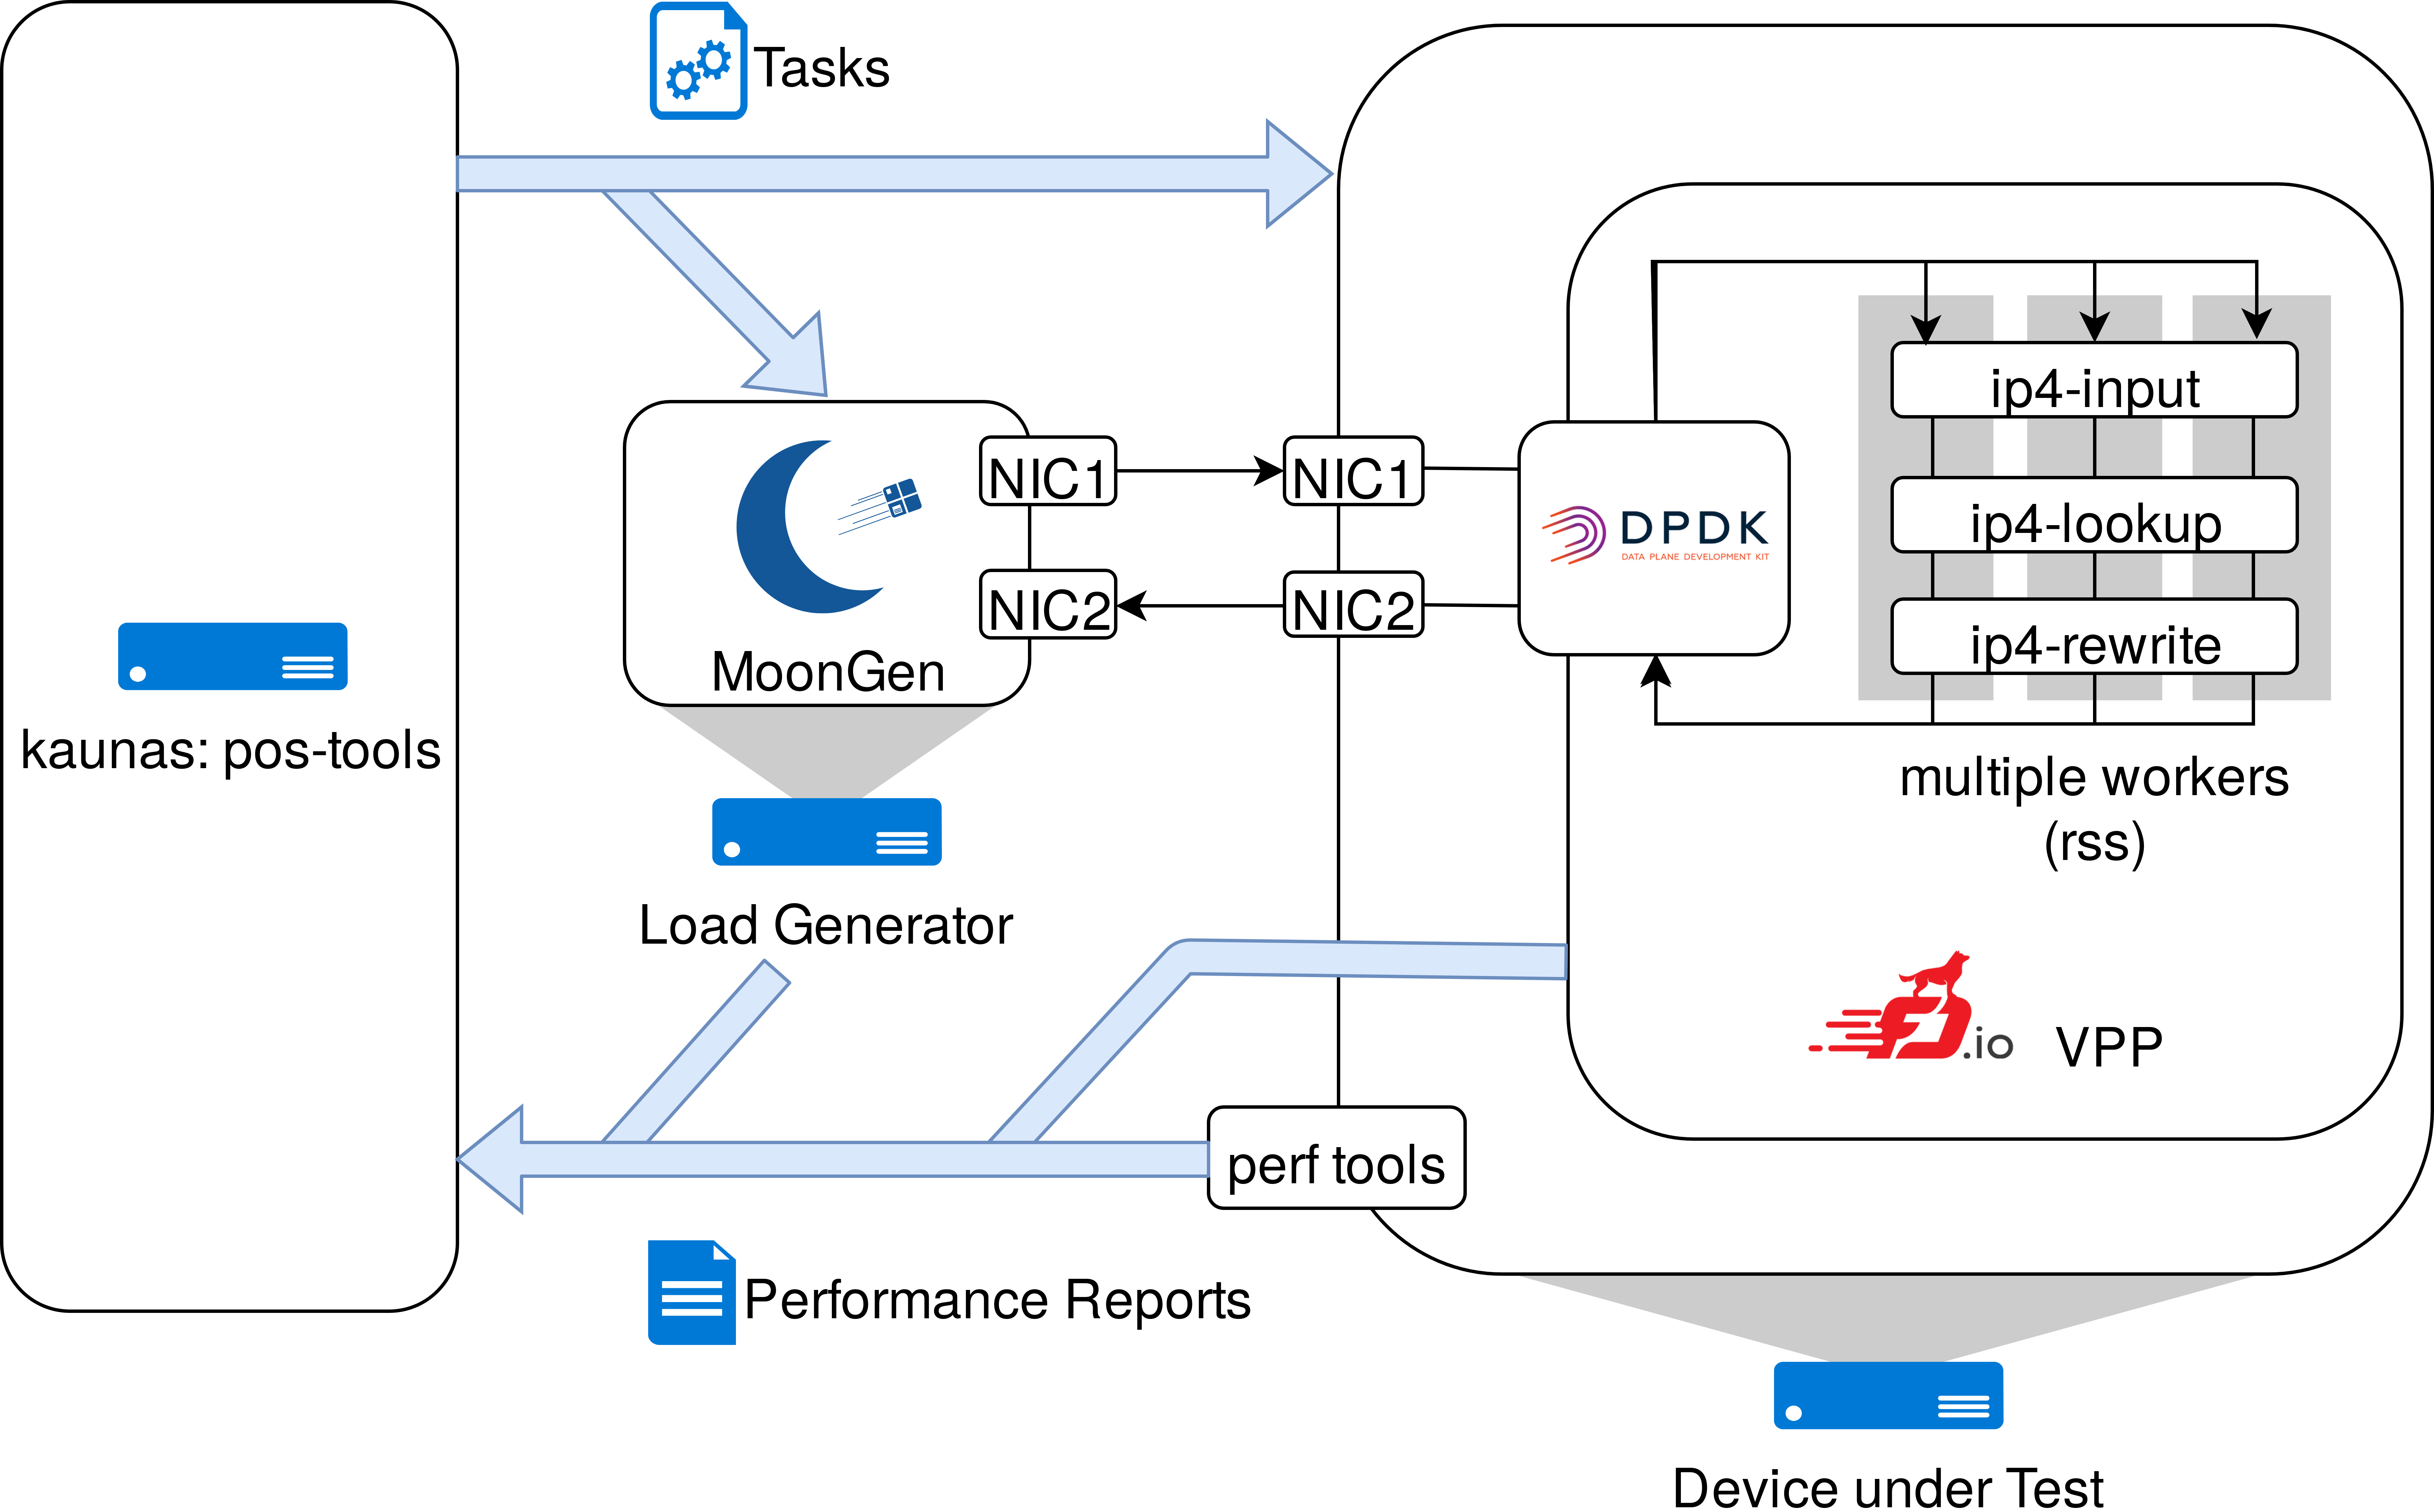
\includegraphics[width=\linewidth]{pics/topology.png}
\caption{Experiment setup for testing VPP with "kaunas" management server, loadgen and DUT}
\label{setup}
\end{figure}


\subsection{Bottlenecks}

\paragraph{Physical Link Speed}
\label{sec:linkspeed}

% - in many cases: 
% 	- 10GbE

Running VPP in with only one worker, the pysical link speed was never
the limiting factor. Usually this is 10GbE in this paper. Only with
multiple worker scenarios the 10Gb/s mark is quickly reached. A simple
way to address this is by testing with bidirectional traffic - sending
load to both of DUT's NIC's and expecting VPP to forward it to both
NIC's again. This way, the load on a single CPU core to be tested can
be doubled, without actually requiring faster links. Other options are
to reduce CPU clock speed or increase the cpu load artificially on a
per-packet basis, in order to create another, even more limiting
bottleneck on the CPU.


\paragraph{Loadgen Speed}

% - loadgen speed
% 	- can saturate a 10GbE link with minimum sized ethernet frames for all tests conducted (14.88mpps)

Another limiting factor could be the load generator's speed of
generating load. MoonGen, the loadgen used for this paper, can
saturate a 10GbE link with minimum sized ethernet frames for all tests
conducted. For a simple unidirectional 10GbE link this results in
14.88mpps \cite{emmerich2015assessing}.

% TODO: remove this if not relevant to the paper: 

Using faster 40GbE with Intel XL710 NICs showed a soft throughput
limit of about 22.81mpps (min. frame size, unidirectional, standard
deviation: 0.22). This was observed with an Intel E5-2620 v3
(2.40GHz). This limit varies when increasing the frame size. Because
reducing the CPU clock speed by 10\% or 50\% results in 12\% and
52\% smaller packet rate, it can be assumed, that this bottleneck lies
within the load generator.

\paragraph{Internal Bandwidth}

% pci bandwidth

Inside the DUT there is first of all the PCI bandwidth. All tested
NIC's are connected by a PCIe 2.0 x8 link with a max transfer rate of
32Gbit/s per direction. In theory a 40GbE link could exceed this
transfer rate. Because the tests in this paper are only done with
small packet sizes, the maximum reached packet generation rate of
around 22.8mpps results in significantly less than 32Gbit/s. For
bigger frame sizes, the PCI bandwidth will become a limiting factor
for 40GbE links.

% ram bandwidth

Sencondly the ethernet frames have to be moved to the main memory. The
test systems use DDR3 memory. It typically supports between 1333 MT/s
(the 10GbE system) or 2133 MT/s (40GbE system) transmitting 64bit per
message. This results in a transfer rate of 85 GBit/s and 136 GBit/s.
This should be sufficient for 10GbE networking, 40GbE links
require at least DDR3-2133 memory. 

\paragraph{CPU time per Packet}

One of the biggest bottlenecks is the CPU time spent per packet, as a
single core can't saturate a 10GbE link. The following subsections
describe how this issue is dealt with in VPP.


% TODO:
% - vpp's cpu cycles: branch prediction, cycles/packet
% - memory latency: latency increases cpu time, caches can improve latency


\subsection{NICs with DPDK and VPP}

For VPP to utilize NIC's up to their specified line rate, it relies on
\Ac{dpdk}. This introduces a few noteworthy optimizations:

\paragraph{RSS (Receive Side Scaling)}

When the NIC recieves a packet, it can be configured to hash over
specified packet header fields to assign the packet to a recieving
queue. The idea is, to efficiently separate for example different ip
traffic flows early which can then be processed by several VPP workers
concurrently and independently. \cite{linguaglossa2017high}

\paragraph{Zero-Copy}

Because memory bandwidth is actually limited, it is important not to
move frames around unnecessarily. Therefore the NIC copys the recieved
frames to memory shared with VPP which is their final fixed
location. \cite{linguaglossa2017high}

\paragraph{Busy Polling}

Newer VPP versions have options to be notified about new packets in
the shared memory via interrupts - or, better suited for high
performance applications, vpp workers can be busy polling.

% TODO
% vpp's multithreading model: hqos, worker, main thread
% placement

\subsection{Packet Processing Graph}

% - modularity, feature rich
%	- visualize the parsing done in the first step as in the vpp paper and explain 
% 		bridging only: ip header parsing slowdown behaviour

VPP's packet processing is defined by the packet processing graph.
Figure \ref{nodegraph} illustrates selected packet paths important for
this paper. Depending on the plugins and configuration in place, this
graph can be customized for example to replace specific software
functions with hardware accelerators. Depending on the initial packet
parsing which happens in the "dpdk-input" and "l2-input" nodes, the
packets traverse the graph over their respective paths.

\paragraph{xconnect}

Static layer 2 connections between physical links (xconnect) are
parsed and passed through the dpdk-, ethernet- and l2-input nodes and
only use the l2-output node to be sent to the target device.

\paragraph{Bridging}

With bridged configurations, packets are treated the same as xconnect
traffic, but there is an additional l2-fwd node which looks up the
destination in the layer 2 \Ac{fib}. Packets for this node are
processed by \lstinline|l2fwd_node_inline| implemented
\lstinline|vpp/src/vnet/l2/l2_fwd.c|.

\paragraph{IPv4}
\label{sec:headerparsing} 

The ip4 path shares it's packet header parsing with the layer 2
processing graph. After it's parsing of a \Ac{udp} packet, the
ip4-lookup and ip4-rewrite nodes implemented by the
\lstinline|ip4_lookup_inline| and the \lstinline|ip4_rewrite_inline|
function in \lstinline|vpp/src/vnet/ip/ip4_forward.c| take care of
looking up the next-hop destination and rewriting the packet header.
Their predecessing node (ip4-input) is also predecessor for other ip4
protocol nodes like for example ICMPv4. A lot of the header parsing
happens before the ip4-input node though, even if this information may
not be needed for the followup nodes.

\paragraph{IPv6}

The ip6 packet processing path differs completely from the previously
discussed paths, because it implements it's own parsing in the
ip6-input node. For lookup and forwarding purpose, there follow an
ip6-lookup and an ip6-rewrite node, similar like the ip4 path. Those
nodes are implemented by the \lstinline|ip6_lookup| and the
\lstinline|ip6_rewrite| function in
\lstinline|vpp/src/vnet/ip/ip6_forward.c|.

\begin{figure}[!ht]
\noindent\hspace{0.5mm}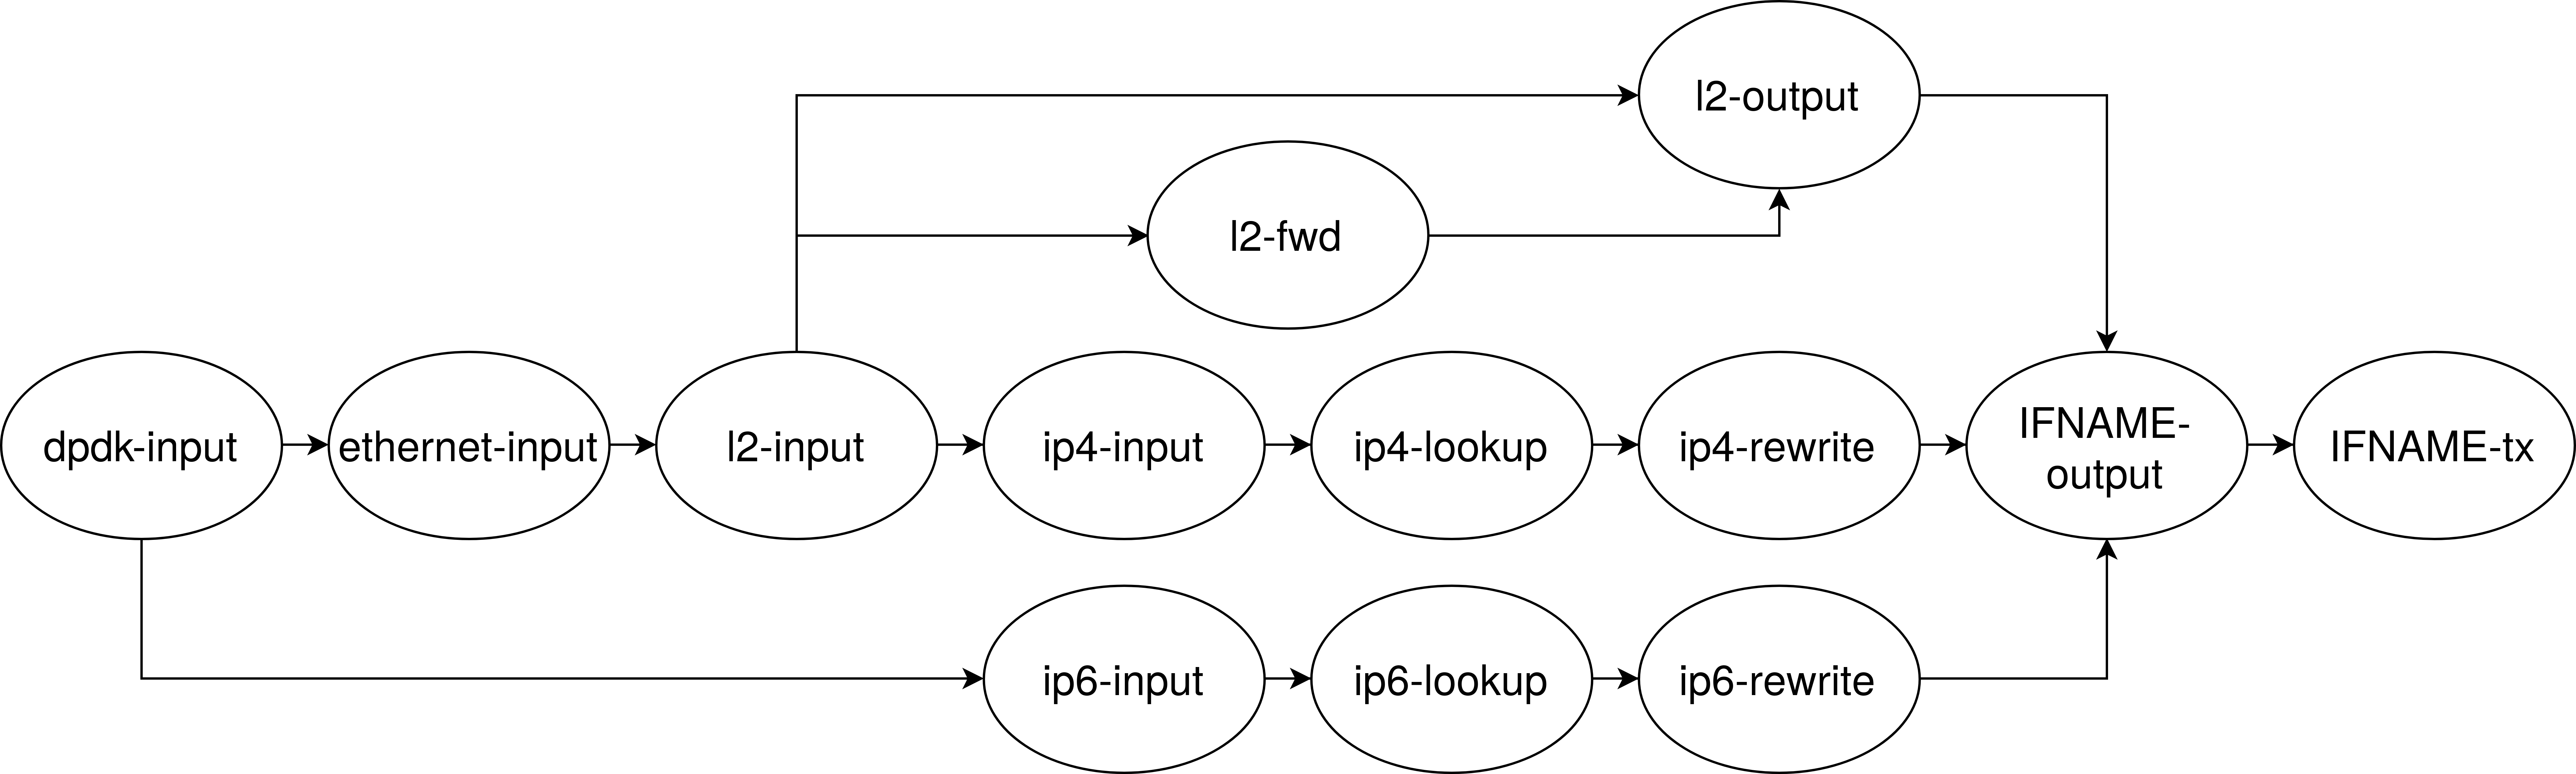
\includegraphics[width=\linewidth]{pics/vpp-nodes-horizontal.png}
\caption{VPP packet processing graph for xconnect, bridging, ip4 routing and ip6 routing. Other paths are left out. }
\label{nodegraph}
\end{figure}

 
\subsection{VPP's forwarding datastructures}

VPP implements several datastructures for their packet forwarding. A
BiHash table is used for the layer 2 \Ac{fib} and the ip6 \Ac{fib}
(\lstinline|vpp/src/vppinfra/bihash*|) \cite{vppwiki:bihash}. IPv4 \Ac{fib}
lookups use a mtrie (\lstinline|vpp/src/vnet/ip/ip4_mtrie.h|).

% There is a  All of them are used to heavily utilize the CPU's cache.

% TODO compare to fastclick's fastest table https://github.com/tbarbette/fastclick/wiki/RangeIPLookup

\paragraph{l2-fib}

For packets reaching the l2-fwd node, the destination lookup is done
for example by \lstinline|l2fib_lookup_4| in
\lstinline|vpp/src/vnet/l2/l2_fib.h|. 

Each lookup takes a 64 bit \lstinline|l2fib_entry_key_t| containing
the mac address and the bridge domain index of the incoming interface.
It returns a 64 bit \lstinline|l2fib_entry_result_t| with the relevant
destination information. 

% one entry cache in l2fib_lookup

\paragraph{ip4-fib}

% hashset vpp/vppinfra/hash.*

% show ip fib and ip4fib functions vpp/src/vnet/fib/ip4_fib.c
% contains ip4_fib_t def.

% ip4-lookup node vpp/src/vnet/ip/ip4_forward.c
% used mtrie: vpp/src/vnet/ip/ip4_mtrie.*

% ip_adjencency_t contains all information about the next hop
% vpp/src/vnet/adj/adj.h

The ip4 lookup is implemented by \lstinline|ip4_fib_table_lookup| in
\lstinline|vpp/src/vnet/fib/ip4_fib.h|. The \Ac{fib} struct
\lstinline|ip4_fib_t| contains two data structures. A list of hash
tables (implemented in \lstinline|vpp/vppinfra/hash.h|), one for each
ip prefix length, which is only used for \Ac{cli} status creation and
to enforce unique inserts. The second data structure is used by the
ip4-lookup node for ip4 \Ac{fib} lookups. The mtrie lookup results in
an adjecency index which is then used by the ip4-rewrite node to
rewrite the destination. Therefore the rewrite node gets the
\lstinline|ip_adjacency_t|\footnote{\lstinline|ip_adjecency_t| is
defined in \lstinline|vpp/src/vnet/adj/adj.h|} information from the
respective adjecency vector according to the adjecency index.

% ip4_lookup_inline prefetch header and frame for next packet badge

\paragraph{ip6-fib}

The ip6 \Ac{fib} lookup itself is done by the ip6-lookup node and
implemented by \lstinline|ip6_fib_table_fwding_lookup| in
\lstinline|vpp/src/vnet/fib/ip6_fib.h| and uses the BiHash table for
lookups in the ip6-lookup node. The lookup returns an 32 bit adjecency
index which will be used by the ip6-rewrite node to get the next
packet destination from the \lstinline|ip_adjencency_t| vector, just
like the ip4-rewrite node does.

% ip4_lookup_inline prefetch header and frame for next packet badge

% table size problems

\subsection{Vectorization}

% - vectorization
% 	- low level optimization for caches
%	- more efficient instruction cache usage?
%	- VLIB_FRAME_SIZE

Vectorization referres to \Ac{vpp} collecting incoming packets in
batches. The input batch size is defined at compile time by
\lstinline|VLIB_FRAME_SIZE| and per default set to 256. This is only
the maximum size though. When packets don't arrive fast enough,
batches are closed and submitted to the processing graph, before the
size limit is reached. Nodes which classify packets might split input
batches allow packets to traverse to different subsequent nodes. In
this case the batch size shrinks further.

This procedure reduces the number of \textit{instruction cache misses}, because
a new node and it's associated function is loaded into the cache only
once for every batch, instead of once per processed packet, as long as
the node is small enough to fit in the cache. The node switching
overhead is therefore shared among all packets in a batch.

Additionally input batching allows for better \textit{data prefetching}. When
each packet traverses the whole graph in a single run, nodes never
know what data the next node will need to be prefetched. With input
batching a single node processes many similar packets in a row and can
thus efficiently prefetch the data it needs for the next packets of
the current batch. Only the first few packets won't be prefetched.

Comparing input batching to \textit{FastClick batching} there are two major
differences: "Nodes in FastClick implicitly process packets
individually, and only specific nodes have been augmented to also
accept batched input" \cite{linguaglossa2017high}. Additionally
\Ac{vpp} has better optimized buffer management and allocation for
input batching for example through reuse of already allocated buffers.
\cite{linguaglossa2017high}

Furthermore the packet batch entering a node can be processed in
batches, too. The packet processing function of a graph node may take
typically up to four packets as parameters to process them
simultaniously. This results in the minimum
\lstinline|VLIB_FRAME_SIZE| beeing four. Not all nodes implement this
feature, sometimes called "\textit{multi-loop}" though, because not
all processing functions profit from it: While the profit in the
xconnect processing path is negligible, the \Ac{ip4} lookup node is
23\% faster with quad loop than with single loop processing. The
\Ac{ip6} lookup node is only 5\% faster.


\subsection{Collected Data}

% why used testing methods: latency, throughput, perf/cache-misses

For buil

For \cite{linguaglossa2017high} the vpp nodes were extended to collect hardware stats for all processing functions individually which allowes for good insights. Because of time constraints this was not done in this paper. Instead this paper simply uses this asd

% Analyzes and assesses several possible approaches that solve the problem





\chapter{Methodology}
\label{sec:methodology}


% \subsection{?implementational details of testing software? (pos, bash, moongen lua)}


% Analyzes and assesses several possible approaches that solve the problem

% why used testing methods: latency, throughput, perf/cache-misses

In this paper the performance of \Ac{vpp} is quantified by throughput
and latency which can be measured by the MoonGen
\cite{emmerich2015moongen} load generator. To help identifying
bottlenecks and limiting factors, \Ac{perf} is used to measure metrics
like cache misses and clock cycle counts. Furthermore \Ac{vpp}'s error
counters are collected after each run, to detect problems in the
packet processing tests.


\section{Measurement Results}

% methods of metric retrieval

% moongen 

\subsection{MoonGen (Throughput and Latency)} 

% TODO talk about threading

The \Ac{dut} sends test traffic using Moongen. There is a lua script
determining MoonGen's behaviour for generating layer 2 ethernet
packets, another one for layer 3 \Ac{ip4} packets, one for \Ac{ip6}
packets and one for \Ac{vxlan} packets. All but the latter can be
given command line parameters to cap the packet rate, change the
packet size, the destinations, the sources and the amount of
destinations to send to.

Additionally the scripts grant \Ac{vpp} some warmup time: Only when
the first packet is successfully forwarded, the actual test begins.
This is necessary, because \Ac{vpp} v18.10 tends to drop packets in
the interface-tx node for a few seconds when it is not warmed up which
could drasically distort the average throughput and latency. After the
other components have settled into the high load situation which takes
around a second, the throughput average stays about constant and can
thus be properly described by the average and standard deviation.

To measure the latency, occasional, timestamped packets are sent by
MoonGen between the load generating packets. This is used to calculate
average and standard deviation and create a histogram of latencies.


\subsection{\Ac{perf}}

\paragraph{perf-stat} 

The command \lstinline|perf stat| is used to attatch to the
\lstinline|vpp_main| process. This allows collection of hardware
counter information about different types of cache events, cpu cycles
used etc. The stats of all children are added up to the main thread's
ones.

\paragraph{perf-record/perf-report}
\label{sec:perf}

The command \lstinline|perf record| is used to attatch to the first
worker thread of \Ac{vpp} or if vpp runs singlethreaded, to the main
thread. This records the cpu time spent per function (symbol). It is
important to connect to a thread processing the packet in \Ac{vpp}'s
graph (not necessarily the main process) to get significant results
for identifying performance limiting factors. After the test run, the
record has to be parsed with \lstinline|perf report| to associate
function names to the symbols.

\paragraph{Performance Impact}

Those two tools run during the test and can therefore impact the
\Ac{dut}'s performance. For \Ac{ip4} forwarding the impact can be up
to 8\% decrease from the original packet throughput rate. That's why
the \Ac{perf} tools are only active for graphs showing cache misses or
time spent per function. 


\subsection{\Ac{vpp} Counters: socat}
\label{sec:vppcounters}

Additionally \Ac{vpp} internal counters, usually used for error
counting, are saved into the test's report for test quality assurance
and debugging. The counters can be read via the \lstinline|show
errors|  \Ac{cli} command. Therefore \Ac{vpp} is configured to listen
at a unix file fifo for it's \Ac{cli}. This interface can be
conveniently used with the tool "vppctl" in \Ac{vpp} v18.10 to connect
and interact with the fifo. In earlier versions like v16.09 this tool
worked differently. In order to be able to read those counters
nevertheless, the tool "socat" was used to connect to the \Ac{cli}
fifo file.


\section{Test Procedure}

One test run tests one \Ac{vpp} configuration. After each test run,
\Ac{vpp} is beeing restarted. After each restart, the performance of
\Ac{vpp} varies significantly more than within one testrun. Therefore
in order to get an insight in how spread the variance is, each test
run is repeated 6 times. Only histogram latency measurements rely on a
single run.

As figure \ref{testsequence} shows, the \Ac{dut} and \Ac{loadgen}
first read the remote configuration file, after the management server
has started the test. Afterwards both devices configure the Intel
pstate driver  as described in section \ref{sec:hardware} and the
\Ac{dut} loads the kernel module for the NIC's. Then \Ac{dut} and
\Ac{loadgen} are synchronized as the pre-test \textit{setup is
complete}.

Before starting the new \Ac{vpp} daemon, the old one is killed and
some files which may contain global state are removed. The \Ac{vpp}
daemon will take at most a few seconds to set itself up, so both
devices are synchronized again and MoonGen is already beeing started,
because it's setup takes longer. When MoonGen is set up and starts
it's warmup loadgen-phase, \Ac{vpp} is already online. \textit{20
seconds} after MoonGen started, both systems are \textit{running and
have stabilized}.

Now, after both systems synchronized again, \textit{\Ac{perf} data is
collected} as described in section \ref{sec:perf} for a timespan of 10
seconds. Then both systems synchronize again, \Ac{vpp}'s counters are
queried (section \ref{sec:vppcounters}), MoonGen is killed and after
giving it 10 seconds time to finalize the throughput and latency
histogram, all files containing test results are uploaded to the
management server.

Approximately 43 seconds after the test started, the final
synchronization takes place an the \textit{next run can be started}.

\begin{figure}[!ht]
\noindent\hspace{0.5mm}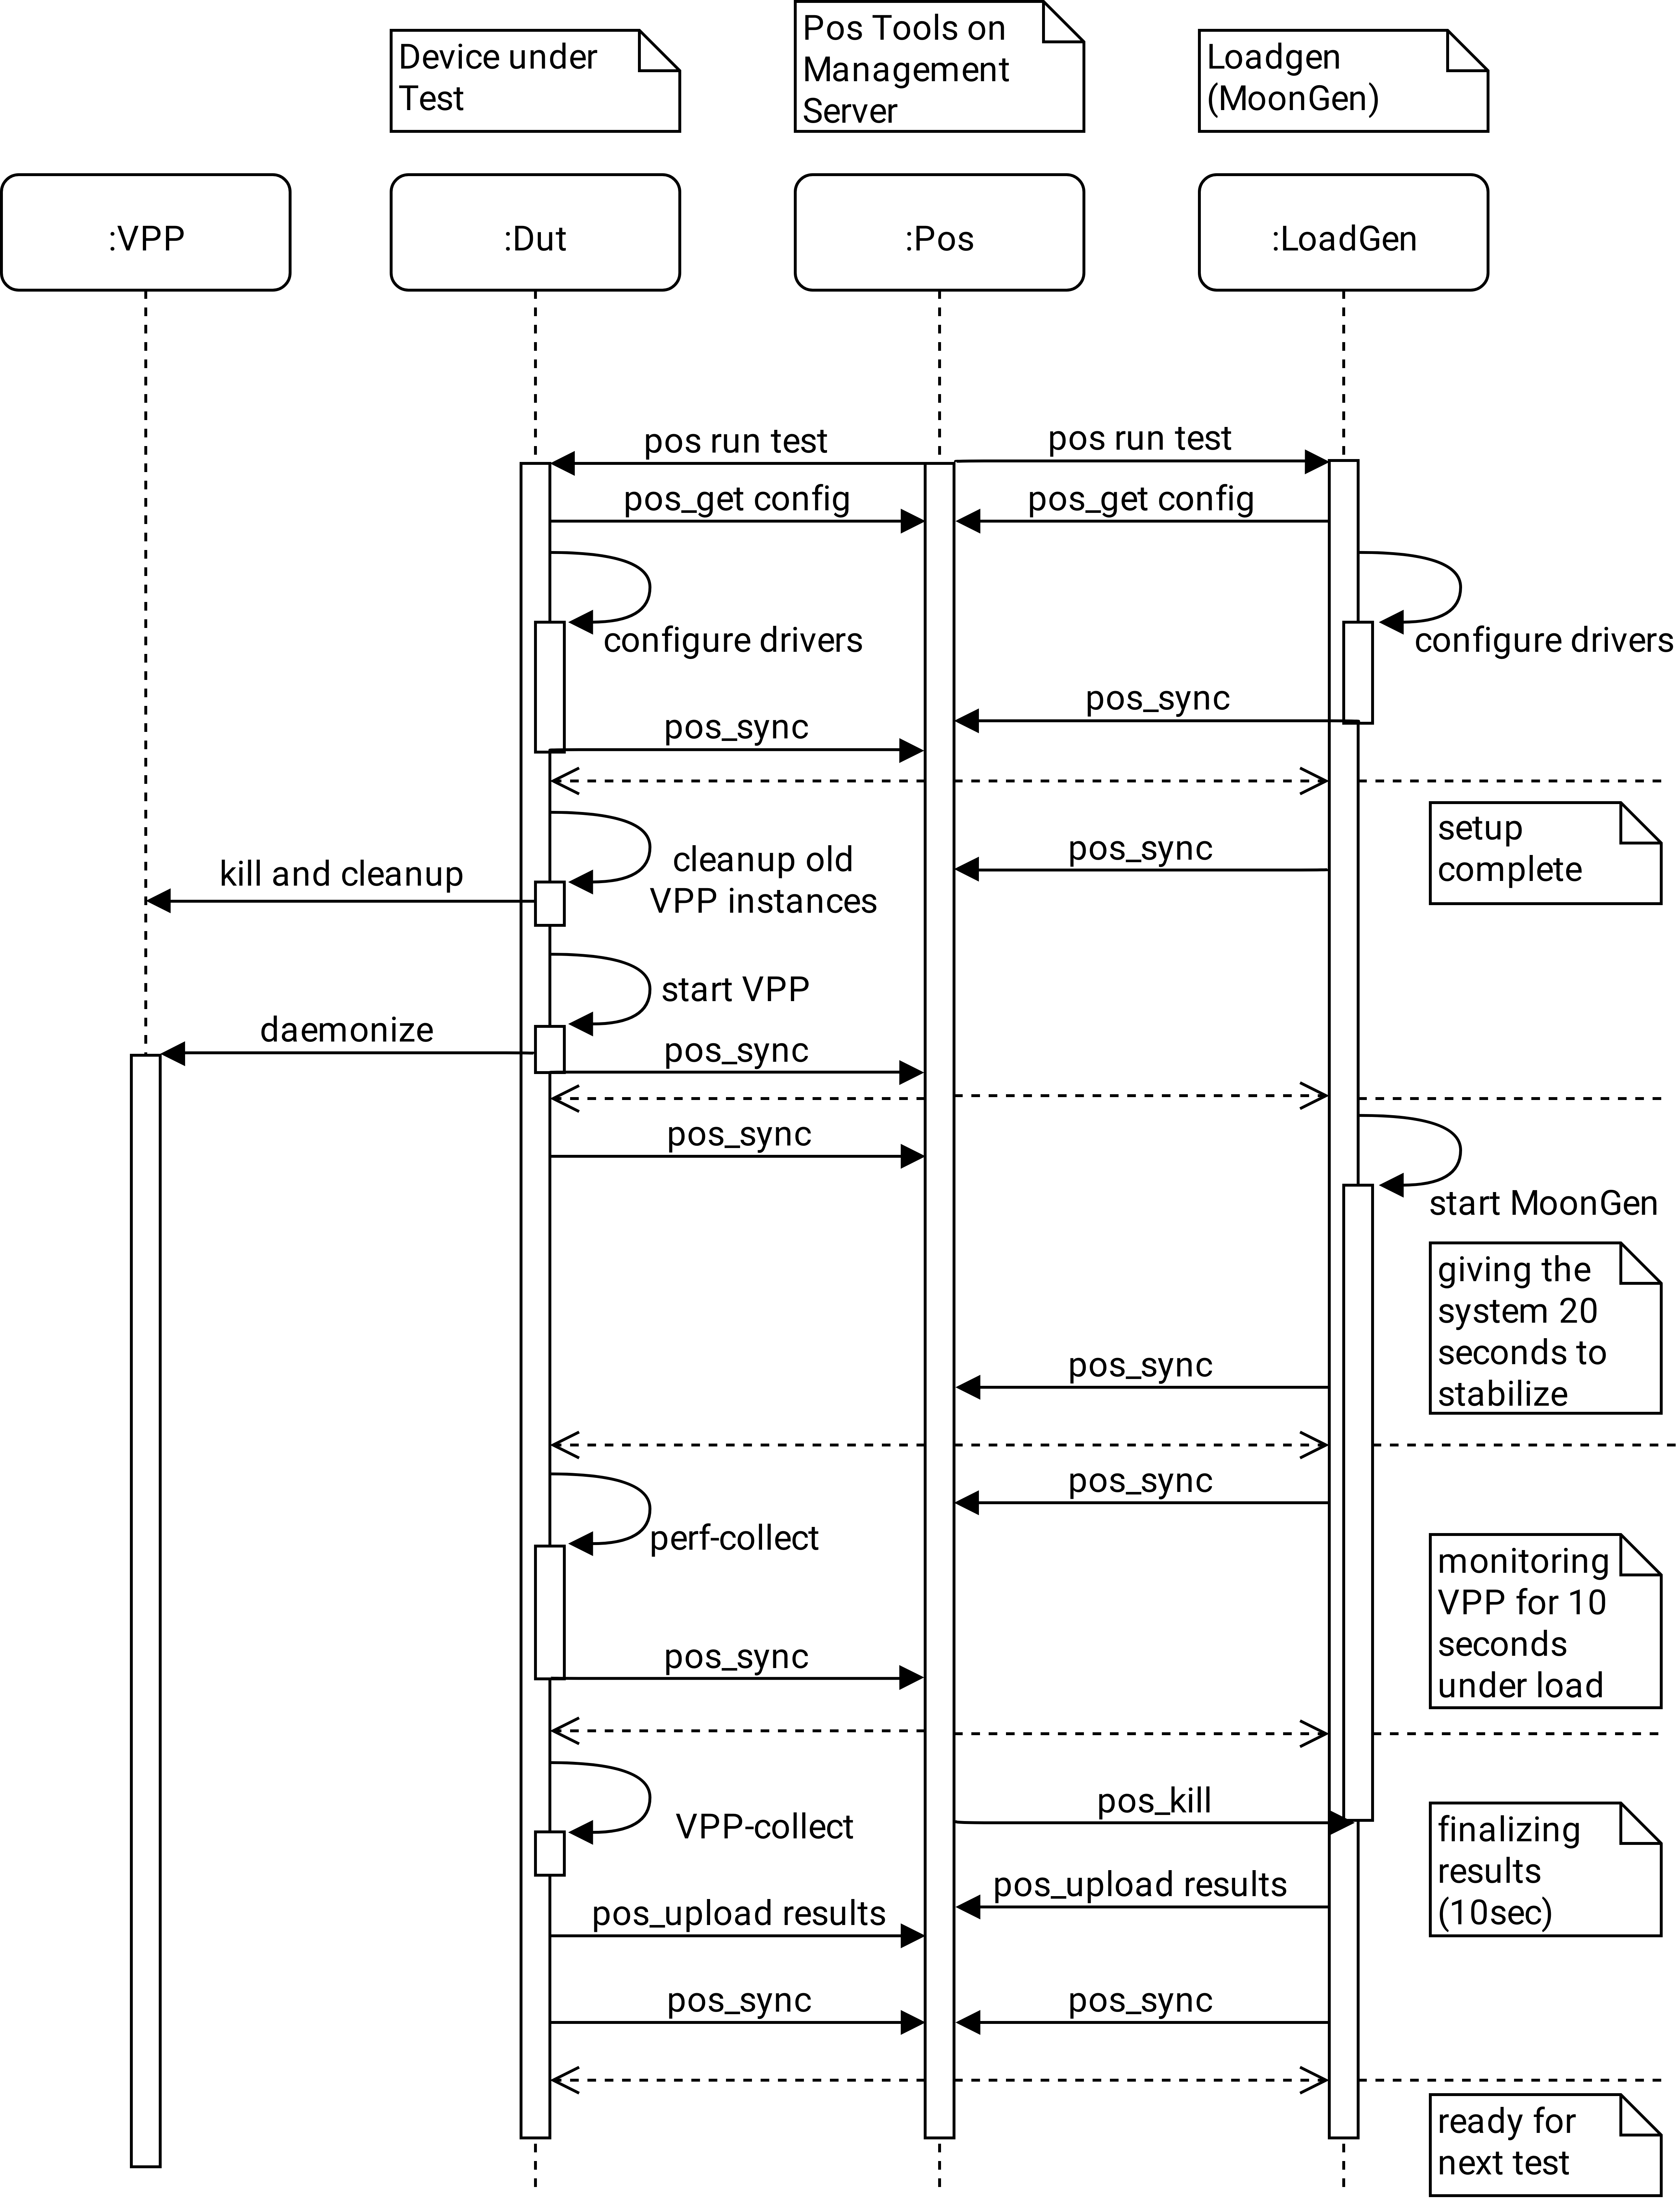
\includegraphics[width=\linewidth]{pics/procedure-sequence.png}
\caption{Sequence of a single testrun. }
\label{testsequence}
\end{figure}


\section{Configuring \Ac{vpp}}

% describe/explain vpp configs/execs

Configuring \Ac{vpp} consists of two steps: Setting the startup
parameters which is done using a \Ac{config} - and executing \Ac{cli}
commands to configure the routing settings on runtime. For the latter
a file containing the \Ac{cli} commands can be specified in the
startup \Ac{config} to be executed. 

The \Ac{vpp} starting scripts used for this paper therefore create
temporary \Ac{config} and \Ac{exec} for example according to the
number of \Ac{ip4} routes specified in the starting script's
parameters. The \Ac{ip4} and \Ac{ip6} scripts also support arbitrary
multicore (-pinning) configurations.

% for the l2fib size tests a plugin was written to add cli support for adding multiple entries with one command.  

Adding millions of \Ac{ip4} or \Ac{ip6} entries to the layer 3
\Ac{fib} is no problem, because the \Ac{cli} already has a command
parameter to add any number of entries through a single command. The
\Ac{cli} commands for the layer 2 \Ac{fib} don't support this though.
Adding millions of entries via the command line would be too time
consuming. That's why this paper uses an own \Ac{vpp} plugin which
extends the \Ac{cli} by a command with this functionality. In terms of
speed it is comparable with the built-in commands.


\section{Tested Scenarios}

For this paper there are many \Ac{vpp} configurations to test several
scenarios:

\paragraph{XConnect} 

The most simple configuration is linking two network interfaces via
cross connect (xconnect). This is a static mapping from one
interface's input to another interface's output and vice versa.

\paragraph{L2 bridging}

For layer 2 switching \Ac{vpp} can create bridge domains. The optional
bridge features mac-learning and mac-aging impact performance when
activated, even when not specifially tested. Other features like
flooding settings have no significant performance impact when not
directly tested. Therefore in section \ref{sec:cpubottleneck} results
are presented with and without the impacting features enabled.

\paragraph{L3 routing}

The \Ac{ip4} and \Ac{ip6} routing tests use multiple routes which all
point to the same destination, conforming RFC2544.

\paragraph{\Ac{vxlan}}

Setting \Ac{vpp} up to encapsulate \Ac{vxlan} packets takes amongh
others the following steps:

\begin{enumerate}
	\item Add a dedicated IP \Ac{fib} table and configure it to route to the \Ac{vxlan} decapsulation endpoint.
	\item Create a bridge domain belonging to the dedicated IP table.
	\item Setup the tunnel using the bridge domain and the dedicated IP table.
	\item Add the new virtual \lstinline|vxlan-tunnel*| interface and all other necessary interfaces to the bridge domain and take care of all of their l2fib entries. 
\end{enumerate}

This means all packets arrive in the bridge domain, are forwarded to
the virtual vxlan-tunnel interface, then encapsulated and sent to the
vxlan-tunnel endpoint via IP.


\section{Testbed Hardware Setup}
\label{sec:hardware}

Test are conducted on different test systems listed in table
\ref{table:hardware}. All of the used systems (the \Ac{loadgen} ones,
too) are configured via the Intel Pstate driver to disable turbo boost
in order to maintain a close to constanct clock speed.

% lscpu
% lshw -C memory
% apt install i2c-tools
% modprobe eeprom
% decode-dimms

\begin{table}[!ht]
	
	\vspace{3ex}
	\begin{tabular}[]{ l | c | c | c }
		DUT & NIC Model & NIC type & RAM \\ \hline
		klaipeda & Intel 82599 & 2x10GbE & DDR3 1333 MHz CL9-9-9-24 \\
		omastar & Intel XL710 & 2x40GbE & DDR4 2133 MHz CL15-15-15-35
	\end{tabular}

	% TODO check this for neccessarity and correctness
	\vspace{2ex}
	\begin{tabular}[]{ l | c | r | r | r | r }
		DUT & CPU @ clock (GHz) & pyhsical cores & L1 cache & L2 cache & L3 cache \\ \hline
		klaipeda & Xeon E3-1230 @ 1.6-3.2 & 4 & 32k & 256k & 8M \\ % 2^23
		omastar & Xeon E5-2630 v4 @ 1.2-2.2 & 10 & 32k & 256k & 25M % 2^
	\end{tabular}

	\caption{\Ac{dut} hardware: CPU model with minimum and maximum clock speed reachable with the Intel Pstate driver without turbo boost, \Ac{nic} model and \Ac{ram} timings}
	\label{table:hardware}
\end{table}

% {details about testbed setup (used servers and configs)}

% cpu config, driver config

% exact test setup description


\chapter{Evaluation and Model}

% show measurement results and explain that headers are parsed for xconnect/bridging even if they are not needed \ref{}

% mention the missing mac addr setting in vpp16.09

% talk about max fib sizes

% mention that for fibs only one via target is used as in rfc defined

% how well does the fantastic memory alignment of vpp work in numa?


\section{CPU as Bottleneck}
\label{sec:cpubottleneck}

Table \ref{bottleneck} presents maximum throughput of all
measured \Ac{vpp} configurations with minimum sized packets using a single \Ac{vpp}
worker. 

The results show, that the computationally least expensive scenario
(xconnect) allows for the highest packet rates. Furthermore we see,
that when reducing the CPU clock speed by 3\%, the number of processed
packets shrinks by around 3\%, too. This indicates, that the CPU
cycles are bottlenecking the packet throughput of \Ac{vpp}.

The same can be seen with other CPU's, too. (TODO reference) This
means for layer 2 configurations the packet throughput $p$ can be
approximated depending on the clock speed $c$ for maxmimum packet
rates $p_{max}$ and the maximum clock speed $c_{max}$:

% f(50%) = 55%
% f(97%) = 98%
% f(100%)= 100%
% f(x) = 0.9 * x + 10

$$ f(c) = (0.9 * \frac{c}{c_{max}} + 0.1) * p_{max} $$

This models approximates for 50\% of the maximum clock speed a
throughput of 55\% of the maximum one. This does not exactly resemble
the expected function $f(c) = \frac{c}{c_{max}} * p_{max}$ (half
the performance at half the clockspeed) which were to be expected if
the CPU cycles were the only limiting factor. This expected behaviour
can be observed though with MoonRoute \cite{chair:architecture} which
indicates another limiting factor, besides CPU
frequency.

% could it be, that vectorization or multi loop gives a base performance boost?

% TODO: automate tests for this table and look at i/d cache misses and perf records

\begin{table}[!ht]
	\vspace{5ex}
	\begin{tabular}[]{ l r r r }
		Scenario & 1.6GHz (50\%) & 3.1GHz (97\%)  & 3.2GHz (100\%) \\ 
		\midrule
		xconnect & 7.34 (56\%) & 12.90 (98\%) & 13.20 (100\%) \\ % stdDev 0.03 0.02 0.12
		l2 bridge no features & 6.69 (55\%) & 11.84 (97\%) & 12.18 (100\%) \\ % 0.01 0.03 0.08
		IPv4 1 route & 6.03 (53\%) & 10.98 (97\%) & 11.28 (100\%) \\ % stdDev 0.01 0.02 0.05
		l2 bridge mac-learn, mac-age & 6.05 (55\%) & 10.84 (98\%) & 11.09 (100\%) \\ % 0.01 0.05 0.02
		IPv6 1 route & 5.38 (53\%) & 9.87 (97\%) & 10.14 (100\%) \\ % 0.01 0.02 0.04
		VXLAN encap & 4.48 (55\%) & 8.15 (99\%) & 8.21 (100\%) \\ % 0.01 0.03 0.39
		IPv4 255k routes & 4.19 (58\%) & 7.06 (97\%) & 7.25 (100\%) \\ % 0.01 0.04 0.07
		IPv6 255k routes & 2.34 (62\%) & 3.72 (98\%) & 3.80 (100\%) \\ % 0.01 0.04 0.02
		\midrule
	\end{tabular}
	\caption{Maximum througput (Mpps) in different scenarios with different CPU frequencies measured on the Xeon E3-1230 system. }
	\label{bottleneck}
\end{table}
% With offered Mpps beeing 100\%, "Relative" is the maximum packet throughput in relation to the offered one.


\section{CPU Scaling Model}

Since the CPU is a bottleneck in all tested configurations, the
ability to distribute the load over multiple CPU cores is
essential. Not all \Ac{vpp} configurations support this though.

\Ac{vpp} has two concepts for using multiple cores: It has workers for
simultanous recieving and processing of packets over the processing
graph - and it can be configured to use another set of workers for
proiritized sending of packets (\Ac{hqos} \cite{vppdocs:qos}
\cite{vppdocs:hqosplacement}). Only the first type of worker can be
used to enhance the performance of raw processing throughput though.

Many layer 3 processing nodes such as the \Ac{ip4} and the \Ac{ip6}
processing path do support parallel packet processing using \Ac{rss}
(see section \ref{sec:rss}). For the scaling to have effect, the
packets need different packet headers though, so that \Ac{rss} header
field hashing can assign them to different queues. Using four
different source addresses per queue is sufficient to hit all of them
well.

Layer 2 bridges on the other hand are completely singlethreaded.
Because \Ac{vxlan} needs a bridge to recieve or send layer 2 traffic,
it can't utilize multiple queues, too.

Scaling measurements are conducted with a 10GbE and a 40GbE link with
high and low CPU clock speed. Test begin with \Ac{vpp} in
singlethreaded mode, having main core and worker in the same thread
and continue with using unused physical cores for workers.

As figure \ref{graph:multicore} shows, switching from singlethreaded
mode to a dedicated worker increases throughput slightly, but barely
noticable. Two cores are already enough to saturate the 10GbE link.
The virtual ("hyper threading") cores are used for workers three to
six within the 10GbE system which results in lower performance gain
and even slight performance loss in the end.

Using the 40GbE system at maximum CPU clock two cores can just not
saturate the limits of the \Ac{nic}. Both 40GbE scaling tests show
that for a workers's maximum throughput $w_{t}$ the overall maximum
throughput depending on the number of workers $w$ is $f(w) = w *
w_{t}$. This holds true until line rate is hit at around two and four
workers, respectively (using pysical cores).

At around 20 Mpps the measured throughput can be unstable by around 0.4
Mpps, because of unstable MoonGen packet generation rates. This is
due to the \Ac{nic} performance limit described in section
\ref{sec:40gbelimit}.

% NAY what happens with different flows per core? low flows but high core count?

% simple cpu scaling on klaipeda 10GbE and omanyte 40GbE
% maybe show both with high and low cpufreq
% klaipeda easily saturated with 2 links
% omanyte with lower freq shows good scaling up to 4 cores

% singlethreaded is typically a ~x% slower than main thread and a single worker

% TODO model: cpu bottleneck model does not apply to omastar cpu. adjust? expand model for workers

\begin{figure}[!ht]
\noindent\hspace{0.5mm}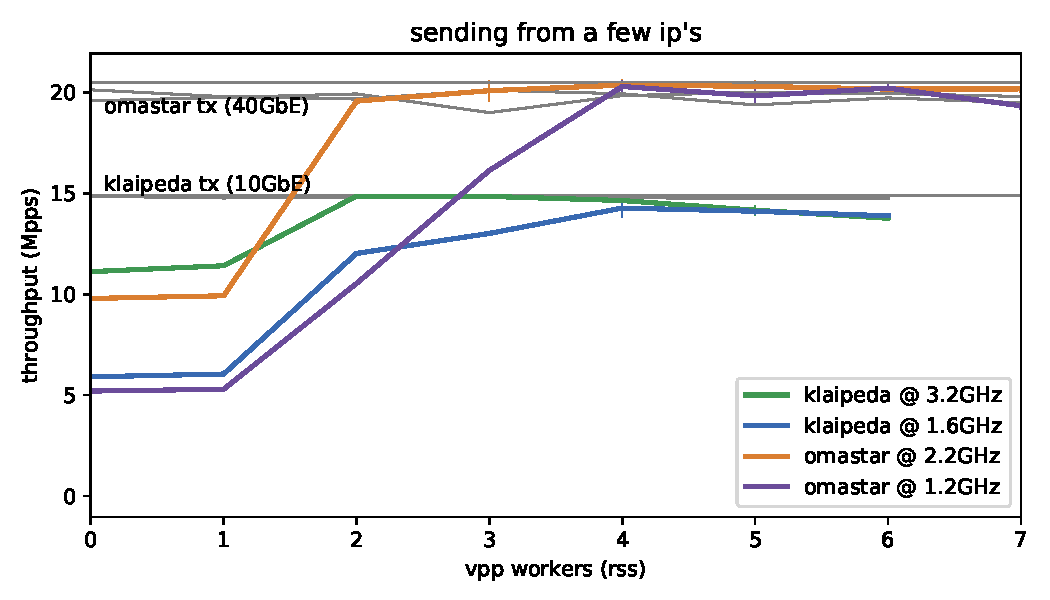
\includegraphics[width=\linewidth]{pics/throughput_summary_multicore.pdf}
\caption{VPP CPU scaling with \Ac{ip4} traffic with 10GbE, 40GbE and different CPU clock speeds. All workers (besides E3-1230 core 3-6) use physical CPU cores. The 40GbE NIC bottlenecks at around 20Mpps (see section \ref{sec:40gbelimit}). }
\label{graph:multicore}
\end{figure}


\section{Lookup Performance Model}

% present measurement results_
% - l2fib
% - ip4
% - ip6
% - v16.09 ip4


\subsection{L2 \Ac{fib}}

The layer 2 \Ac{fib} is tested by configuring \Ac{vpp} with varying
amounts of l2fib entries and sending packets to random destinations
using a single worker.

Figure \ref{graph:l2fib} shows that with only one l2fib entry you get
0.5 Mpps more throughput compared with two l2fib entries. This is due
to the simple caching mechanism of the l2fib-lookup function: It
stores the last looked up information locally, so that when the next
packet goes to the same destination, the local values can be used and
a hash table lookup can be skipped.

From there on there are three key points when the CPU's L1, L2 and L3
cache are full. We can model the BiHash l2fib lookup table takes 64
bit values as input and returns a 64 bit result. Assuming the table
only contains keys and values, the maximum \Ac{fib} size fitting into
cache of $n$ bytes is:

$$ f_{l2fib}(n) = n * \frac{8}{2 * 64} = n * \frac{1}{16}  $$

This formula is used to create the l1, l2 and l3 cache marks in figure
\ref{graph:l2fib} as a upper bound for how many fib entries could fit
into the respective caches. 

As figure \ref{graph:l2fib} shows, the throughput drops before the L1
cache as the L1 cache misses start rising. With the Layer 2 cache mark
the throughput drops further and more CPU time is spent inside the
\lstinline|l2fwd_node| function which does the lookup. Finally before
the layer 3 mark, the respective data cache misses rise, the
throughput drops further and close to 40\% of the CPU time is spent
inside the lookup node.





\subsection{\Ac{ip6} \Ac{fib}}

Figure \ref{graph:ip6fib} shows the results of \Ac{ip6} routing with
different layer 3 \Ac{fib} sizes. It's maximum size is remarkably
smaller compared to the layer 2 \Ac{fib}. Each lookup table result
value is only 32 bit in size. Assuming the table only contains those
values and keys the size of an \Ac{ip6} address, the maximum \Ac{fib}
size fitting into cache of $n$ bytes is:

$$ f_{ip6fib}(n) = n * \frac{8}{128 + 32} = n * \frac{1}{24}  $$

This means for a layer 3 cache size of 8MB ($2^{23}$B) at most 350,000
could fit into it. At this \Ac{fib} size we are off the charts though
and there is no correlating change in throughput. Therefore the model
for layer 2 \Ac{fib}s seem not to apply to \Ac{ip6} \Ac{fib}s.

% TODO there is a change before 4096 in omastar 

% l2 cache size of 256k (2^18) at most 32,768 routes -> right after the big drop

Nevertheless it can be assumed the massive drop in performance from
20,000 \Ac{fib} entries upwards is because of the BiHash table lookups
taking longer because of cache size limitations, since the big drop of
throughput closely correlates to the layer 3 cache misses and the time
spent in the lookup function.







\subsection{\Ac{ip4} \Ac{fib}}
\label{sec:ip4fib}

While the layer 2 \Ac{fib} can contain over $2^{23}$ entries, tests
show that \Ac{vpp} v18.10 stops working with more than 287,743
\Ac{ip4} \Ac{fib} entries. To be able to compare \Ac{vpp} to other
software routers nevertheless, tests conducted with v16.09 show that
this version is able to handle up to around 12,580,000 \Ac{fib}
entries which is well above $2^{23}$.

Figure \ref{graph:ip4fib} and \ref{graph:ip4fiblegacy} show test
results of \Ac{vpp} v18.10 with up to 255,000 entries and of v16.09
with up to 10,300,000 entries. Both show similar behaviour to the
\Ac{ip6} \Ac{fib} tests with one big throughput drop torwards the end
of the graph.

% TODO point out, that index lookup is not the performance issue

\subsection{Lookup Nodes as Bottleneck}

With big lookup tables, the throughput drops a lot with every kind of
lookup table because for every additional CPU cycle spent for the
lookup in relation to the available cycles, the throughput will drop
by the same ratio. Thus the maximum throughput $f$ can be modeled
depending on the relative time $d_{lookup}$ spent in the lookup node
function for a known maximum throughput $t_{max}$ with one or two
routes:

$$ f(x) = t_{max} * ( 1 - d_{lookup} ) $$

The measurements closely resemble this model. They proof that the
lookup is basically exclusively responsible for the performance
decrease of bigger \Ac{fib}s and thus a limiting factor scenarios with
big routing tables.

\begin{figure}[!ht]
\noindent\hspace{0.5mm}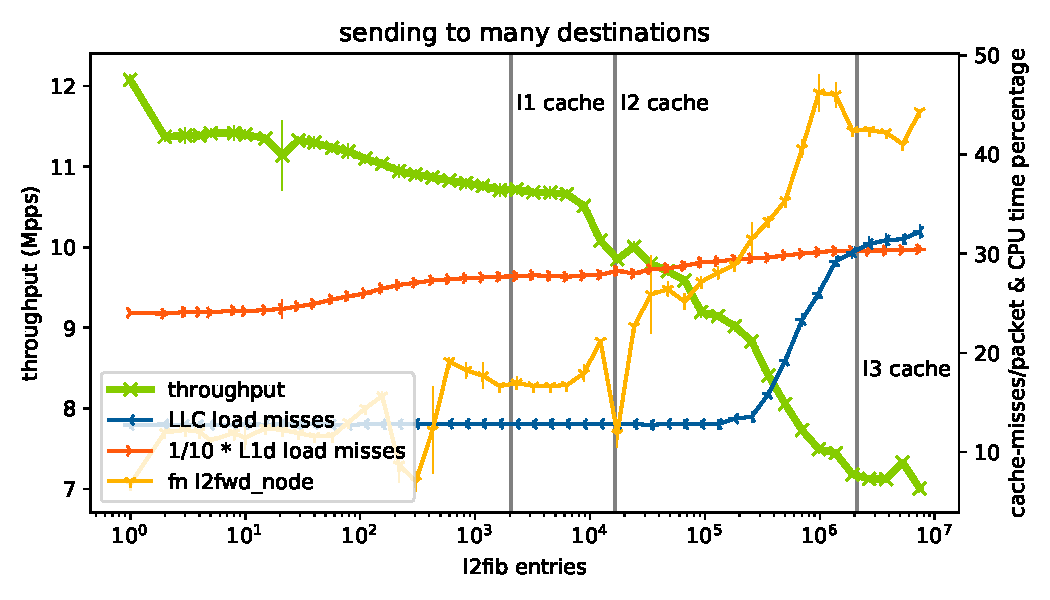
\includegraphics[width=\linewidth]{pics/throughput_l2_throughmac_klaipeda32ghz_v3.pdf}
\caption{Testing \Ac{vpp} v18.10 with different layer 2 \Ac{fib} sizes. Throughput, Layer 1 data cache load misses (devided by 10) and Last Level Cache load misses per packet and the percentage of CPU time spent in selected functions. }
\label{graph:l2fib}
\end{figure}

\begin{figure}[!ht]
\noindent\hspace{0.5mm}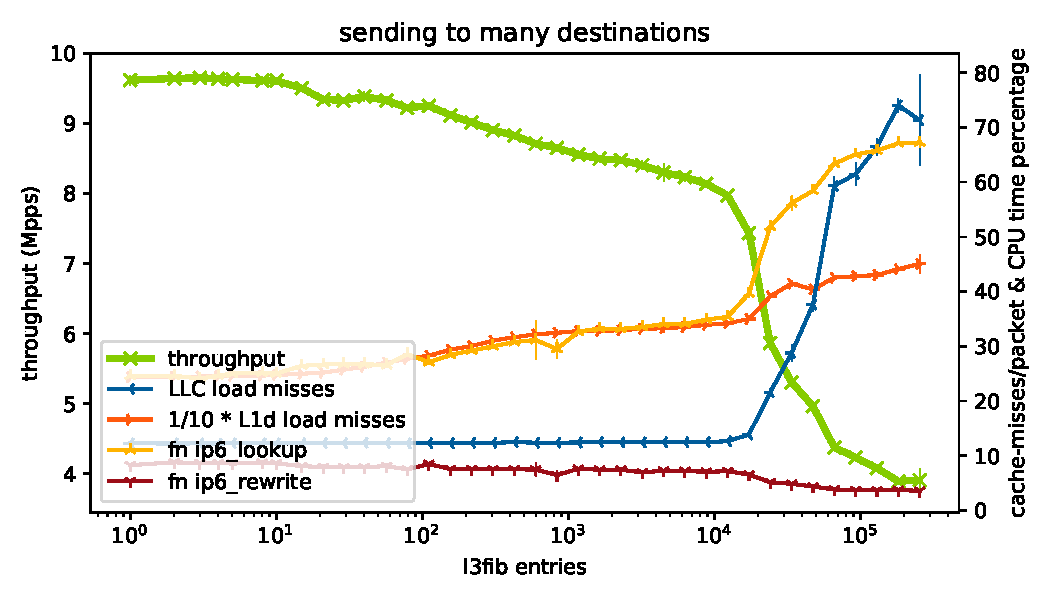
\includegraphics[width=\linewidth]{pics/throughput_l3v6_routes_klaipeda32ghz_v3.pdf}
\caption{Testing \Ac{vpp} v18.10 with different \Ac{ip6} \Ac{fib} sizes. Throughput, Layer 1 data cache load misses (devided by 10) and Last Level Cache load misses per packet and the percentage of CPU time spent in selected functions. }
\label{graph:ip6fib}
\end{figure}

\begin{figure}[!ht]
\noindent\hspace{0.5mm}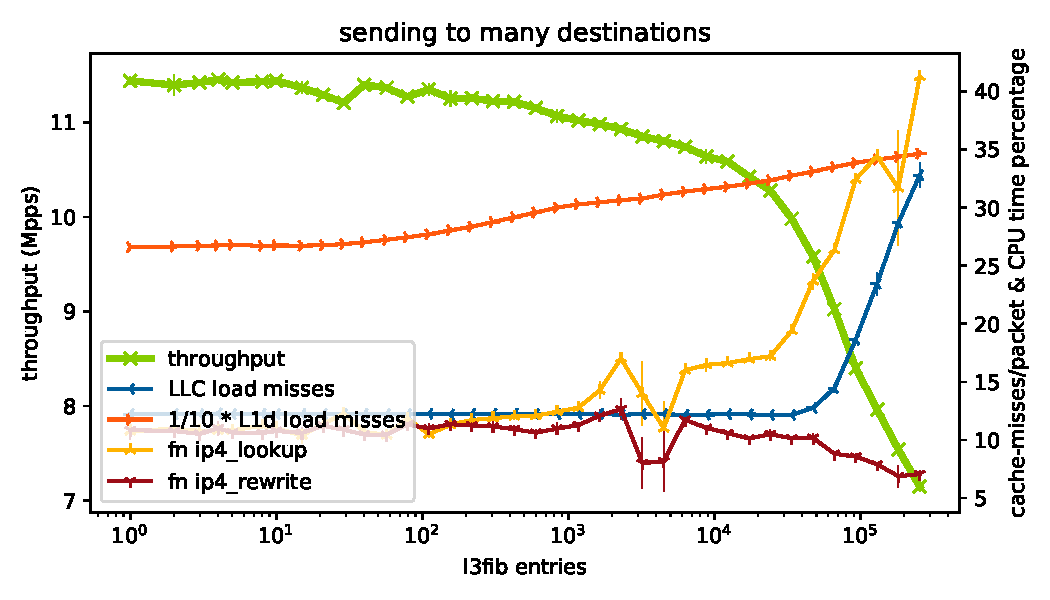
\includegraphics[width=\linewidth]{pics/throughput_l3_routes_klaipeda32ghz_v3.pdf}
\caption{Testing \Ac{vpp} v18.10 with different \Ac{ip4} \Ac{fib} sizes. Throughput, Layer 1 data cache load misses (devided by 10) and Last Level Cache load misses per packet and the percentage of CPU time spent in selected functions.}
\label{graph:ip4fib}
\end{figure}

\begin{figure}[!ht]
\noindent\hspace{0.5mm}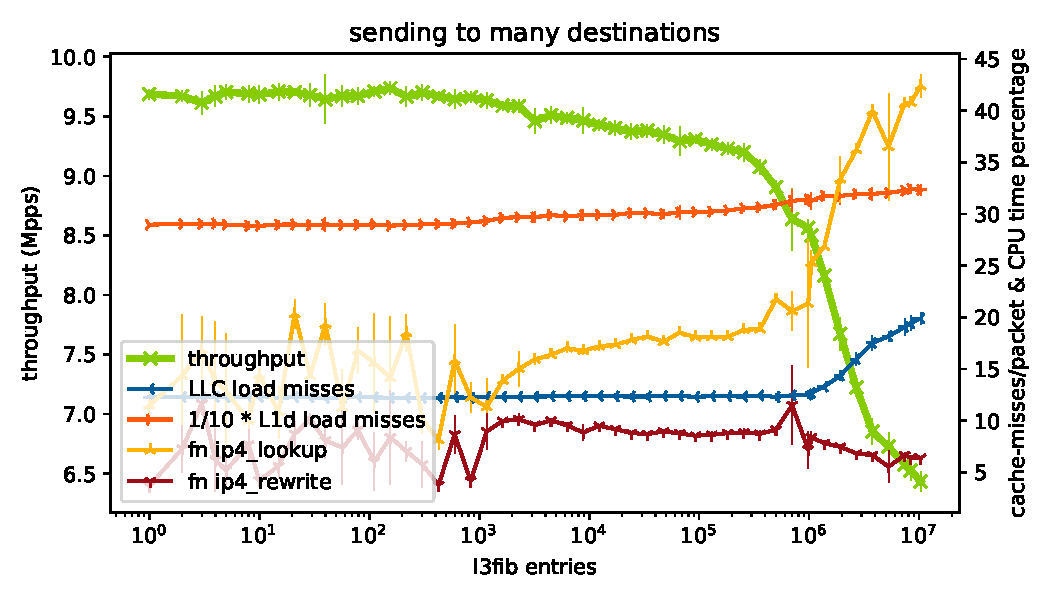
\includegraphics[width=\linewidth]{pics/throughput_l3_routes_klaipeda_v1609_32ghz_v3.pdf}
\caption{Testing \Ac{vpp} v16.09 with different \Ac{ip4} \Ac{fib} sizes. Throughput, Layer 1 data cache load misses (devided by 10) and Last Level Cache load misses per packet and the percentage of CPU time spent in selected functions. }
\label{graph:ip4fiblegacy}
\end{figure}

% model the performance decrease according to causes

% cpu scaling

% TODO fix perf stack plot script

\section{Latencies}

\subsection{Average Latencies}

% TODO: this section refferes to max throughput as NDR

% dropped frames per throughput, latency: avg, 99.999 percentile per throughput

Measuring the latency should be done with reduced offered load,
because when offering the load at full link speed, the average latency
hits a worst case which is orders of magnitude higher than at lower
packet rates. Figure \ref{graph:latencyoverview} shows the average
latency and the packet loss at different packet rates for \Ac{ip4}
routing with 1 and with 255,000 routes. It shows that the latency is
around $\SC{5}{\mu s}$ for low line rates and slowly increases
torwards reaching the maximum throughput. When this maximum is
reached, the packet drop rates immediately go up, because not all
packets can be forwarded. This is also exactly the point where the
latency explodes to around $\SC{600}{\mu s}$ because packet queues
fill up.

The qualitative latency behaviour described in figure
\ref{graph:latencyoverview} between 1 and 255k routes is similar. The
following function can approximate the average latency for different
packet rates $t \in (0, t_{max})$ for a known maximum packet
throughput $t_{max}$. 

$$ l(t) = 59 - 62 * (-\frac{t}{t_{max}}+1)^{\frac{t_{max}}{8t}} $$ 

% this is already said in Latency Distribution

% Generally speaking, an increase in latency with growing load is
% expected, because of \Ac{vpp}'s vectorization. As explained in section
% \ref{sec:vectorization}, the lower the packet rate, the earlier
% batches are closed and processed even if the batch is hardly filled.
% Therefore individual packets have to wait less time at average to be
% processed.

\begin{figure}[!ht]
\noindent\hspace{0.5mm}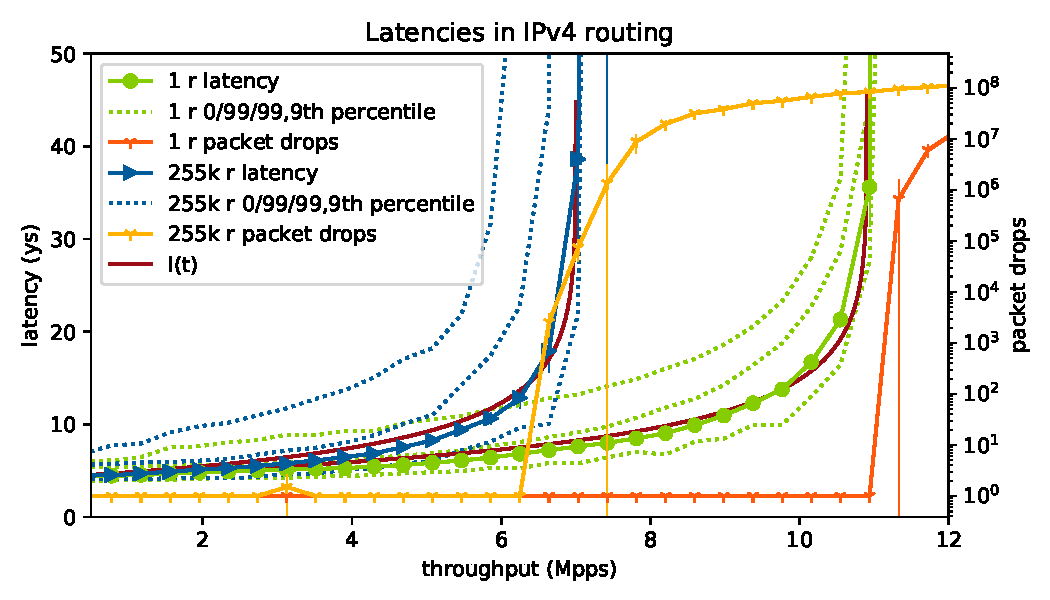
\includegraphics[width=\linewidth]{pics/latencies_per_throughput_summary_ip4.pdf}
\caption{Latencies in $\mu s$ and packet drops of \Ac{ip4} routing with a single route (1 r) and 255k routes (255k r). }
\label{graph:latencyoverview}
\end{figure}

\subsection{Latency Distribution}

Figure \ref{graph:latencyhistogram} shows histograms of latency for
\Ac{ip4} routing at approximately 10\%, 50\% and 90\% of the maximum
throughput rate. It shows that under very low load the latency
distribution peaks in the beginning. Later on the distribution can be
approximated as a standard distribution but with growing average and
standard deviation. The reason for this is lies within \Ac{vpp}
closing the batches as long as the packet processing is not stressed
to it's limits (see \ref{sec:vectorization}). This results in earlier
processing of packets at low loads and explains why at 50\% of the
maximum load the latency is the same, even though the lookup load is
different. \cite{linguaglossa2017high}


% histogram
% ip4 1route low, 90\% and max load (0.1, 0.5, 0.9)
% ip4 255routes low, 90\% and max load

% 1r 7.8mpps 50% 8502.523457,		 35% 992.510538			28% ixgbe_xmit_pkts 31736245724cycles
% 1r 10.86mpps 90% 25631.480224,	100% 2790.657240

% 255r 5.87mpps 50% 11283.178205,2072.334996		18% ixgbe_xmit_pkts 31488860702
% 255r 7.28mpps 90% 911243.365558,9960.445080

% serialization takes 30% of time -> ( cycles/s / packets/s ) * 0.3 * cycles/s => 0.3 * latency = 3ys tx time
% => tx time is approximately latency stdDev
% Each batch spends 30\% of it's time in the tx node. This means the first packet will be sent approximately 0.3*latency before the last one. This is the latency. 
% As figure \ref{graph:latencyhistogram} shows, this holds true for high packet throughputs when batches are always nearly full. For very low throughput the histogram does not resemble the standarddeviation and indicates that many packets get their very own vector. Thus the big spike at the beginning of the distribution. 

% TODO: test traffic patterns. 
% TODO: check back l2 bridge histograms which were more interesting.

\begin{figure}[!ht]
\noindent\hspace{0.5mm}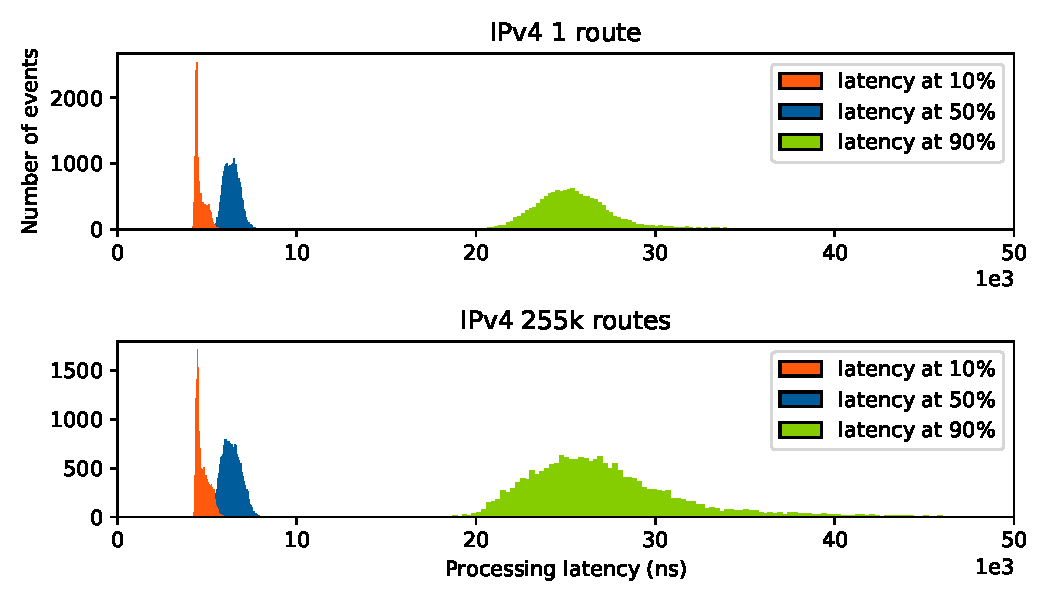
\includegraphics[width=\linewidth]{pics/latency_histogram_overview_ip4.pdf}
\caption{Latency histogram for \Ac{ip4} routing with a single route and 255k routes at approximately 10\%, 50\% and 90\% of the maximum throughput rate. }
\label{graph:latencyhistogram}
\end{figure}


% \subsection{Bottleneck Analysis}

% - fib: memory cache speed
% - cpu cycles
% - other hardware bottleneck? but this was already written about in analysis


\section{Comparison}

Tests showed that there are big performance differences even between
\Ac{vpp} versions. While v16.09 is slower when using litte \Ac{ip4}
routes, it doesn't have the maximum \Ac{fib} size of 255k which is
exceptionally low compared to other software routers. Generally
speaking though, it is at least twice as fast as Click DPDK and has
similar performance to FastClick DPDK. \Ac{vpp} v18.10 beeing 1.2 mpps
faster than FastClick DPDK indicates better optimizations and higher
potential for \Ac{vpp} v18.10 - but for routing tables with 30,000 to
1,000,000 entries FastClick DPDK has a very clear lead.

% vectorization of vpp and fastclick and not the others

\begin{table}[!ht]
	\vspace{5ex}
	\begin{tabular}[]{ l r r r }
		Implementation	 & FIB sizes & Mpps		& Relative \\ 
		\midrule
		MoonRoute		 & 1		 & 14.6		& 100\% \\
		MoonRoute		 & $2^{20}$	 & 14.2		& 97\% \\
		MoonRoute		 & $2^{24}$	 & 11.6		& 79\% \\
		VPP v18.10		 & 1		 & 11.6		& 79\% \\
		FastClick DPDK	 & 1		 & 10.4 	& 72\% \\
		FastClick DPDK	 & $2^{20}$	 & 10.4 	& 72\% \\
		VPP v16.09		 & 1		 & 9.7	 	& 71\% \\
		VPP v16.09		 & 255k		 & 9.2	 	& 63\% \\
		VPP v16.09		 & $2^{20}$	 & 8.5	 	& 58\% \\
		VPP v18.10		 & 255k		 & 7.2	 	& 50\% \\
		VPP v16.09		 & $2^{23}$	 & 6.5	 	& 45\% \\
		Click DPDK		 & 1		 & 4.3 		& 29\% \\
		Click DPDK		 & $2^{20}$	 & 4.2 		& 28\% \\
		Linux 3.7		 & 1		 & 1.5 		& 11\% \\

		\midrule
	\end{tabular}
	\caption{Comparison of maximum \Ac{ip4} forwarding throughput with a single worker on the Xeon E3-1230 system (see table \ref{table:hardware}). Non-VPP results are from \cite{chair:architecture} and are conducted on the same system. }
	\label{table:comparison}
\end{table}

% TODO: moonroute, fastclick and click need citation

% \subsubsection{TODO sections:}

% Compare own measurements with figure 5+6 regarding latencies (linux, microtik, freebsd) of revisiting benchmarking methodology for interconnected devices.
% + frame losses (fig. 3):

\chapter{Conclusion}

FastClick and \Ac{vpp} are both fast software routers which vectorize
packets during processing and are close to each other performance
wise. MoonRoute on the other hand has a significant performance
advantage over both of them, being 20-30\% faster at routing.

While the performance of \Ac{vpp} v18.10 starts dropping at around 20
\Ac{fib} entries, \Ac{vpp} v16.09 can hold its highest performance
with up to 200 \Ac{ip4} \Ac{fib} entries. 

Reaching the maximum number of entries, \Ac{vpp}'s throughput nearly
halves with \Ac{vpp} v18.10 only supporting up to around 287,000
\Ac{ip4} \Ac{fib} entries. For this number of routing table entries it
is remarkably slower than FastClick with $2^{20}$ entries, even though
it is slightly faster with little table entries.

The best advantage of \Ac{vpp} over its competitors is its feature
richness. Its during runtime configurable packet processing graph
offers for example different tunneling protocols. Settings allow to
move the main thread to a dedicated CPU core which in turn allows live
inserts of 255k routing table entries with a temporary throughput
impact of less than a percent.

Although \Ac{vpp} performs badly with very big routing tables, its
modularity in combination with the rich options to connect it to
virtual machines, containers or local high performance applications,
make it a well choice for building virtual networks for highly
virtualized environments or implementation of \Ac{vnf}.

Next research steps could include more specific benchmarks regarding
behavior on receiving control packets or \Ac{ip6} specific
benchmarking methodology like RFC 5180 \cite{rfc5180}. Furthermore the
performance change over different \Ac{vpp} versions can be analyzed
closer by testing a version between 16.09 and 18.10 and the latest
v19.01 which was just released during the creation of this paper.
Especially the code changes leading to the performance differences and
how for example FastClick achieves its high performance with many
routes is of interest.

% TODO: this has to sound better

% more next steps: 
% - compare more vpp versions v19.01!
% - code based comparison of lookup table: v16.09, v18.10, fastclick
% - Understand where latency is introduced. model/plain why latency
%   per load graph looks like it does (read the relevant code)
% - try to elaborate a better upper bound throughput model as in: 
%   "Performance Exploration of Software-based Packet Processing Systems"
% 	- test with different cpus
% - test in virtualized scenarios
%   - take a look at open daylight / open flow / open stack to find out 
%     if there are good solutions to the terrible configuration problem 
% - test "smart" numa memory alignment
% - warmup time: somebody mentioned, that dpdk gets slower (less average throughput), 
%   when there is too little time between two busy polls
% - more interesting l2 histograms?


%\appendix
%\chapter{Supplementals}
%\chapter{Appendix}

foo


\printacronyms[heading=chapter,name=List of acronyms]
\clearpage
\pagestyle{thesischapter}

\cleardoublepage
\printbibliography[heading=bibintoc]

%\cleardoublepage
\clearpage
\pagestyle{empty}
%\mbox{}
%\clearpage

\end{document}


